% 41039 Programming 1 revision; shared style copied from the established Week 4 deck.
\documentclass[aspectratio=169]{beamer}
\makeatletter

\usepackage{lmodern}
\usepackage{booktabs}
\usepackage{array}
\usepackage{graphicx}
\usepackage{xcolor}
\usepackage{listings}
\usepackage{pifont}
\usepackage{enumitem}
\usepackage[most]{tcolorbox}
\usepackage{tikz}
\usetikzlibrary{shapes.geometric, arrows.meta, positioning}

% Beamer's default enumerate label expands to itself once enumitem takes the optional
% argument, and TeX runs out of input stack. An explicit label breaks the loop.
\setlist[enumerate]{label=\arabic*.}
\setlist[itemize]{label=\usebeamertemplate{itemize item}}

\definecolor{bkblue}{RGB}{0,70,140}
\definecolor{bktitlebg}{RGB}{64,116,169}
\definecolor{codebg}{RGB}{244,246,249}
\definecolor{codecmt}{RGB}{110,120,130}
\definecolor{codegray}{RGB}{110,120,135}
\definecolor{codestr}{RGB}{150,60,20}
\definecolor{badred}{RGB}{185,40,40}
\definecolor{goodgreen}{RGB}{20,125,70}
\definecolor{srcgrey}{RGB}{105,115,128}

\usetheme{default}
\useinnertheme{rounded}
\setbeamertemplate{navigation symbols}{}

\setbeamercolor{titlelike}{bg=bktitlebg,fg=white}
\setbeamercolor{frametitle}{fg=bkblue,bg=}
\setbeamercolor{author}{fg=bkblue}
\setbeamercolor{institute}{fg=bkblue}
\setbeamercolor{section in toc}{fg=bkblue}
\setbeamerfont{frametitle}{size=\Large,series=\mdseries}
\setbeamerfont{title}{size=\Large,series=\bfseries}
\setbeamerfont{subtitle}{size=\normalsize,series=\bfseries}

\setbeamertemplate{frametitle}{%
  \vspace*{0.35em}%
  \begin{minipage}[b]{0.84\textwidth}%
    \usebeamerfont{frametitle}\usebeamercolor[fg]{frametitle}\insertframetitle%
  \end{minipage}\hfill%
  \begin{minipage}[b]{0.10\textwidth}%
    \raggedleft
\includegraphics[height=0.75cm]{bk-logo.png}%
  \end{minipage}\\[0.1em]%
  {\color{bkblue}\rule{\textwidth}{0.7pt}}%
}

\setbeamercolor{footbar}{bg=bkblue,fg=white}
\setbeamertemplate{footline}{%
  \begin{beamercolorbox}[wd=\paperwidth,ht=2.1ex,dp=1.1ex,leftskip=.3cm,rightskip=.3cm]{footbar}%
    \tiny\insertshorttitle\hfill\insertframenumber{}/\inserttotalframenumber%
  \end{beamercolorbox}%
}

\newcommand{\keyline}[1]{\vfill\begin{center}\textcolor{bkblue}{\textbf{#1}}\end{center}\vspace*{0.2em}}
\newcommand{\hd}[1]{\textbf{#1}}
\newcommand{\code}[1]{\texttt{#1}}
\newcommand{\srcline}[1]{{\color{srcgrey}\scriptsize #1\par}}
\newcommand{\srclink}[2]{\href{#1}{\texttt{#2}}}
\newcommand{\badlabel}[1]{\textcolor{badred}{\ding{55}~\textbf{#1}}}
\newcommand{\goodlabel}[1]{\textcolor{goodgreen}{\ding{51}~\textbf{#1}}}
\newcommand{\neutrallabel}[1]{\textcolor{bkblue}{\textbf{#1}}}
\newcommand{\timing}[2]{\hfill{\small\textcolor{bkblue}{\textbf{#1 \textbullet{} #2}}}}
% a blank to be filled in, numbered so the word bank can be checked against it
\newcommand{\blank}[1]{\underline{\hspace{1.1em}\textbf{(#1)}\hspace{1.1em}}}
\newcommand{\yes}{\textcolor{goodgreen}{\ding{51}}}
\newcommand{\no}{\textcolor{badred}{\ding{55}}}

% --- Stack and heap pictures (Draw it) --------------------------------------
\tikzset{
  sframe/.style={draw=bkblue, thick, fill=codebg, rounded corners=2pt, inner sep=4pt,
    font=\scriptsize\ttfamily, align=left, anchor=north west},
  ftitle/.style={font=\scriptsize\sffamily\bfseries, text=bkblue, anchor=south west},
  cell/.style={draw=bkblue, fill=white, font=\scriptsize\ttfamily, minimum width=0.62cm,
    minimum height=0.5cm, inner sep=1pt},
  atitle/.style={font=\scriptsize\ttfamily, text=bkblue, anchor=south west, inner sep=1pt},
  ref/.style={-{Stealth[length=5pt]}, thick, draw=bkblue!85!black},
  hd/.style={font=\small\sffamily\bfseries, text=bkblue},
}

\hypersetup{colorlinks=true, urlcolor=bkblue, linkcolor=bkblue}

% --- Question box: what the room is being asked --------------------------
\newtcolorbox{discussionbox}[1]{
  title=\textbf{#1}, coltitle=bkblue, colback=white, colframe=bkblue,
  colbacktitle=bkblue!10, boxrule=1pt, arc=3pt,
  left=6pt, right=6pt, top=4pt, bottom=4pt
}
% --- Answer box: revealed after they have committed to an answer ---------
\newtcolorbox{contextbox}[1]{
  title=\textbf{#1}, coltitle=white, colback=bkblue!5, colframe=bkblue,
  colbacktitle=bkblue!80, boxrule=0.6pt, arc=3pt,
  left=6pt, right=6pt, top=4pt, bottom=4pt
}

\lstdefinestyle{code}{
  basicstyle=\ttfamily\scriptsize,
  keywordstyle=\color{bkblue}\bfseries,
  commentstyle=\color{codecmt}\itshape,
  stringstyle=\color{codestr},
  backgroundcolor=\color{codebg},
  frame=leftline, framerule=1.2pt, rulecolor=\color{bkblue},
  xleftmargin=1.1em, framexleftmargin=1.1em,
  framexrightmargin=0.4em, framextopmargin=3pt, framexbottommargin=3pt,
  showstringspaces=false, columns=fullflexible, keepspaces=true,
  breaklines=true, aboveskip=0.6em, belowskip=0.6em,
}
\lstdefinestyle{bad}{style=code, rulecolor=\color{badred}, backgroundcolor=\color{badred!4}}
\lstdefinestyle{good}{style=code, rulecolor=\color{goodgreen}, backgroundcolor=\color{goodgreen!5}}
\lstset{style=code}
% listings' Python predates 3.10; teach it the soft keywords and constants this deck uses
\lstdefinelanguage{Py}[]{Python}{morekeywords={match,case,elif,True,False}}

\setbeamertemplate{title page}{%
  \vspace*{0.5em}
  \begin{centering}
    \begin{beamercolorbox}[sep=8pt,center,rounded=true,shadow=false]{title}
      \usebeamerfont{title}\inserttitle\par
      \ifx\insertsubtitle\@empty\else
        \vskip0.4em{\usebeamerfont{subtitle}\insertsubtitle\par}
      \fi
    \end{beamercolorbox}
    \vskip1.0em
    
\includegraphics[height=1.7cm]{bk-logo.png}
    \vskip1.0em
    {\usebeamercolor[fg]{author}\usebeamerfont{author}\insertauthor\par}
    \vskip0.5em
    {\usebeamercolor[fg]{institute}\usebeamerfont{institute}\insertinstitute\par}
    \vskip0.6em
    {\usebeamerfont{date}\insertdate\par}
  \end{centering}
}




\title[41039 Programming 1 --- Revision of Week 7]{41039 Programming 1}
\subtitle{Revision of Week 7: Lists and generics}
\author{Dr. Xuan-Bach Le\\ \small\texttt{le.xuan.bach@hcmut.edu.vn}}
\institute{\small Faculty of Computer Science and Engineering, HCMUT}
\date{September Session 2026}
\AtBeginSection[]{\begin{frame}{Outline}\tableofcontents[currentsection]\end{frame}}
\begin{document}

\begin{frame}{}
\titlepage
\end{frame}

\begin{frame}{How the revision session works}
\begin{discussionbox}{A recap before the next lecture}\small Write an answer before the reveal. Explain the state change, rule or contract that makes it follow. These are practice questions, with no new assessment requirements.\end{discussionbox}
\begin{columns}[T,onlytextwidth]
\column{0.48\textwidth}
\raggedright
\neutrallabel{Part 1: on your own}\begin{itemize}\small\item 6 short questions\item About 90 seconds per question\item Java and Python; name the language first\end{itemize}
\column{0.48\textwidth}
\raggedright
\neutrallabel{Part 2: teams of 3 or 4}\begin{itemize}\small\item Draw the model\item Spot the errors\item Predict the output\item Write and test the code\end{itemize}
\end{columns}
\keyline{A result needs a reason. A repair needs a counterexample.}
\end{frame}

\section{On your own}

\begin{frame}[fragile]{1. Changing a resizable list}
\srcline{Java 8 excerpt: main statements and supporting types; commit to an outcome before the reveal.}
\begin{columns}[T,onlytextwidth]
\column{0.62\textwidth}
\raggedright
\begin{lstlisting}[style=code,language=Java]
import java.util.ArrayList;
ArrayList<String> names = new ArrayList<String>();
names.add("An");
names.add("Mai");
names.add(1,"Linh");
names.set(0,"Binh");
System.out.println(names);
System.out.println(names.size());
\end{lstlisting}

\column{0.34\textwidth}
\raggedright
\begin{onlyenv}<1>\begin{discussionbox}{Your answer}\small What is the complete output? Which line or rule decides it?\end{discussionbox}\end{onlyenv}
\begin{onlyenv}<2>\begin{contextbox}{Answer}
\begin{lstlisting}[style=code]
[Binh, Linh, Mai]
3
\end{lstlisting}
\scriptsize\raggedright add at an index inserts; set replaces. Three elements remain.
\end{contextbox}\end{onlyenv}
\end{columns}

\end{frame}

\begin{frame}[fragile]{2. The comparable Python operations}
\srcline{Python 3; commit to an outcome before the reveal.}
\begin{columns}[T,onlytextwidth]
\column{0.62\textwidth}
\raggedright
\begin{lstlisting}[style=code,language=Py]
names = ["An", "Mai"]
names.insert(1, "Linh")
names[0] = "Binh"
print(names)
print(len(names))
\end{lstlisting}

\column{0.34\textwidth}
\raggedright
\begin{onlyenv}<1>\begin{discussionbox}{Your answer}\small What is the complete output? Which line or rule decides it?\end{discussionbox}\end{onlyenv}
\begin{onlyenv}<2>\begin{contextbox}{Answer}
\begin{lstlisting}[style=code]
['Binh', 'Linh', 'Mai']
3
\end{lstlisting}
\scriptsize\raggedright Python lists offer the same insert/replace distinction, with different syntax.
\end{contextbox}\end{onlyenv}
\end{columns}

\end{frame}

\begin{frame}[fragile]{3. Remove an index or remove a value?}
\srcline{Java 8 excerpt: main statements and supporting types; commit to an outcome before the reveal.}
\begin{columns}[T,onlytextwidth]
\column{0.62\textwidth}
\raggedright
\begin{lstlisting}[style=code,language=Java]
import java.util.ArrayList;
import java.util.Arrays;
ArrayList<Integer> values = new ArrayList<Integer>(Arrays.asList(4,1,4));
values.remove(1);
values.remove(Integer.valueOf(4));
System.out.println(values);
\end{lstlisting}

\column{0.34\textwidth}
\raggedright
\begin{onlyenv}<1>\begin{discussionbox}{Your answer}\small What is the complete output? Which line or rule decides it?\end{discussionbox}\end{onlyenv}
\begin{onlyenv}<2>\begin{contextbox}{Answer}
\begin{lstlisting}[style=code]
[4]
\end{lstlisting}
\scriptsize\raggedright The index removal leaves [4,4]; the value removal deletes only the first 4.
\end{contextbox}\end{onlyenv}
\end{columns}

\end{frame}

\begin{frame}[fragile]{4. Safe filtering produces a new list}
\srcline{Python 3; commit to an outcome before the reveal.}
\begin{columns}[T,onlytextwidth]
\column{0.62\textwidth}
\raggedright
\begin{lstlisting}[style=code,language=Py]
values = [1, 2, 2, 3, 4]
kept = [value for value in values if value % 2 == 1]
print(kept)
print(values)
\end{lstlisting}

\column{0.34\textwidth}
\raggedright
\begin{onlyenv}<1>\begin{discussionbox}{Your answer}\small What is the complete output? Which line or rule decides it?\end{discussionbox}\end{onlyenv}
\begin{onlyenv}<2>\begin{contextbox}{Answer}
\begin{lstlisting}[style=code]
[1, 3]
[1, 2, 2, 3, 4]
\end{lstlisting}
\scriptsize\raggedright Filtering leaves the source unchanged and keeps both order and only the matching values.
\end{contextbox}\end{onlyenv}
\end{columns}

\end{frame}

\begin{frame}[fragile]{5. A reusable, type-safe box}
\srcline{Java 8 excerpt: main statements and supporting types; commit to an outcome before the reveal.}
\begin{columns}[T,onlytextwidth]
\column{0.62\textwidth}
\raggedright
\begin{lstlisting}[style=code,language=Java]
Box<String> label = new Box<String>("tea");
Box<Integer> count = new Box<Integer>(3);
System.out.println(label.get() + " " + count.get());
class Box<T> {
    private final T value;
    Box(T value) { this.value = value; }
    T get() { return value; }
}
\end{lstlisting}

\column{0.34\textwidth}
\raggedright
\begin{onlyenv}<1>\begin{discussionbox}{Your answer}\small What is the complete output? Which line or rule decides it?\end{discussionbox}\end{onlyenv}
\begin{onlyenv}<2>\begin{contextbox}{Answer}
\begin{lstlisting}[style=code]
tea 3
\end{lstlisting}
\scriptsize\raggedright The class is reused with two types while each individual box retains a checked element type.
\end{contextbox}\end{onlyenv}
\end{columns}

\end{frame}

\begin{frame}[fragile]{6. The same FIFO contract with deque}
\srcline{Python 3; commit to an outcome before the reveal.}
\begin{columns}[T,onlytextwidth]
\column{0.62\textwidth}
\raggedright
\begin{lstlisting}[style=code,language=Py]
from collections import deque
queue = deque(["An", "Mai"])
print(queue.popleft())
print(list(queue))
\end{lstlisting}

\column{0.34\textwidth}
\raggedright
\begin{onlyenv}<1>\begin{discussionbox}{Your answer}\small Predict the output. Which Java list provides addLast/removeFirst? Why would repeated get(i) on that list be expensive?\end{discussionbox}\end{onlyenv}
\begin{onlyenv}<2>\begin{contextbox}{Answer}
\begin{lstlisting}[style=code]
An
['Mai']
\end{lstlisting}
\scriptsize\raggedright popleft removes An, and Mai remains waiting. Java LinkedList provides addLast/removeFirst. Finding an arbitrary index requires traversing links, so repeatedly accessing every index can take quadratic time. Prefer sequential iteration for that access pattern.
\end{contextbox}\end{onlyenv}
\end{columns}

\end{frame}

\section{Team round 1: draw the model}

\begin{frame}{Form teams}
\begin{itemize}[itemsep=0.8em]\item Teams of 3 or 4. One shared sheet, one spokesperson.\item For each challenge, record the result and the reason.\item Rotate the spokesperson. Other teams can challenge an explanation.\item The final task has starter files and a Java/Python solution pair.\end{itemize}\keyline{Discuss first. Commit to an answer. Then compare with the reveal.}
\end{frame}

\begin{frame}[fragile]{Draw it: A list copy and a reference copy}
\begin{columns}[T,onlytextwidth]
\column{0.62\textwidth}
\raggedright
\begin{lstlisting}[style=code,language=Java]
import java.util.*;
List<Integer> a=new ArrayList<Integer>(Arrays.asList(4,1,4));
List<Integer> b=a;
List<Integer> c=new ArrayList<Integer>(a);
b.remove(Integer.valueOf(4));
c.set(0,9);
System.out.println(a);
System.out.println(b);
System.out.println(c);
\end{lstlisting}

\column{0.34\textwidth}
\raggedright
\begin{discussionbox}{Four minutes}\small Draw the object references after the shown operations. Label the important state. Mark what is shared, what changes, or which path handles failure. Predict every output line.\end{discussionbox}
\end{columns}
\par\srcline{\href{../../weeks/week-7.html}{Course website: Week 7}. Complete programs accompany this deck.}

\end{frame}

\begin{frame}[fragile]{Draw it: one answer}
\begin{columns}[T,onlytextwidth]
\column{0.66\textwidth}
\raggedright
\resizebox{\linewidth}{!}{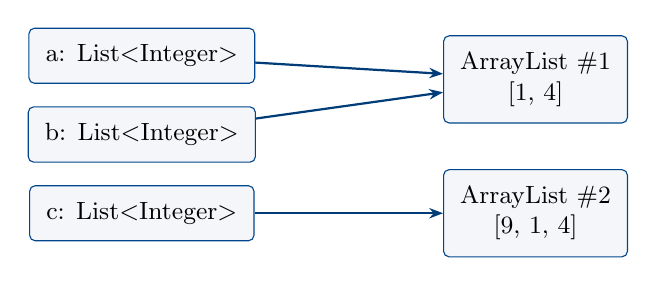
\begin{tikzpicture}
\node[draw=bkblue,rounded corners=2pt,fill=codebg,align=center,inner sep=6pt,font=\small] (a) at (0,0) {a: List\textless{}Integer\textgreater{}};
\node[draw=bkblue,rounded corners=2pt,fill=codebg,align=center,inner sep=6pt,font=\small] (b) at (0,-1) {b: List\textless{}Integer\textgreater{}};
\node[draw=bkblue,rounded corners=2pt,fill=codebg,align=center,inner sep=6pt,font=\small] (c) at (0,-2) {c: List\textless{}Integer\textgreater{}};
\node[draw=bkblue,rounded corners=2pt,fill=codebg,align=center,inner sep=6pt,font=\small] (o1) at (5,-0.3) {ArrayList \#1\\[0pt] [1, 4]};
\node[draw=bkblue,rounded corners=2pt,fill=codebg,align=center,inner sep=6pt,font=\small] (o2) at (5,-2) {ArrayList \#2\\[0pt] [9, 1, 4]};
\draw[ref] (a) -- (o1);
\draw[ref] (b) -- (o1);
\draw[ref] (c) -- (o2);
\end{tikzpicture}}

\column{0.3\textwidth}
\raggedright
\begin{contextbox}{Output}\begin{lstlisting}[style=code]
[1, 4]
[1, 4]
[9, 1, 4]
\end{lstlisting}
\end{contextbox}
\end{columns}
\vspace{0.8em}
\small new ArrayList(a) creates a distinct list container. The elements here are immutable Integer values, so a shallow copy is sufficient for independent changes to list positions.
\par\srcline{\href{../../weeks/week-7.html}{Course website: Week 7}. Complete programs accompany this deck.}

\end{frame}

\section{Team round 2: spot the errors}

\begin{frame}[fragile]{Spot the errors 1: Java (5 min)}
\begin{discussionbox}{Contract}\small Remove one occurrence of target by value, then every 9. Expected final list: [2]. Test target values that differ from their positions.\end{discussionbox}
\begin{columns}[T,onlytextwidth]
\column{0.48\textwidth}
\raggedright
\begin{lstlisting}[style=bad,language=Java,numbers=left,numberstyle=\tiny\color{codegray},firstnumber=1,numbersep=0.7em]
import java.util.*;
public class Broken {
    public static void main(String[] args) {
        ArrayList<Integer> xs=new ArrayList<Integer>(Arrays.asList(9,1,9,2));
        int target=1;
        xs.remove(target);
\end{lstlisting}

\column{0.48\textwidth}
\raggedright
\begin{lstlisting}[style=bad,language=Java,numbers=left,numberstyle=\tiny\color{codegray},firstnumber=7,numbersep=0.7em]
        for(int i=0;i<xs.size();i++) {
            if(xs.get(i)==9) xs.remove(i);
        }
        System.out.println(xs);
    }
}
\end{lstlisting}

\end{columns}

\end{frame}

\begin{frame}[fragile]{Spot the errors 1: answers}
\begin{columns}[T,onlytextwidth]
\column{0.58\textwidth}
\raggedright
\begin{contextbox}{The repairs}\footnotesize\begin{itemize}[itemsep=0.45em]\item \textbf{L6:} An int selects index removal; wrap target to select removal by value. This data initially hides the mistake.\item \textbf{L7:} Removing while increasing i skips an adjacent match after elements shift. Traverse indices backwards.\end{itemize}\end{contextbox}
\column{0.38\textwidth}
\raggedright
\badlabel{Original program}\begin{lstlisting}[style=code]
[9, 2]
\end{lstlisting}
\goodlabel{After the repairs}\begin{lstlisting}[style=code]
[2]
\end{lstlisting}

\end{columns}
\par\srcline{\href{../../weeks/week-7.html}{Course website: Week 7}. Complete programs accompany this deck.}

\end{frame}

\begin{frame}[fragile]{Spot the errors 2: Python (5 min)}
\begin{discussionbox}{Contract}\small Keep odd values in a new list, preserving order and leaving values unchanged.\end{discussionbox}
\begin{columns}[T,onlytextwidth]
\column{0.48\textwidth}
\raggedright
\begin{lstlisting}[style=bad,language=Py,numbers=left,numberstyle=\tiny\color{codegray},firstnumber=1,numbersep=0.7em]
values=[2,2,3,4,4,5]
kept=values
for value in kept:
\end{lstlisting}

\column{0.48\textwidth}
\raggedright
\begin{lstlisting}[style=bad,language=Py,numbers=left,numberstyle=\tiny\color{codegray},firstnumber=4,numbersep=0.7em]
    if value%2==0: kept.remove(value)
print(kept)
print(values)
\end{lstlisting}

\end{columns}

\end{frame}

\begin{frame}[fragile]{Spot the errors 2: answers}
\begin{columns}[T,onlytextwidth]
\column{0.58\textwidth}
\raggedright
\begin{contextbox}{The repairs}\footnotesize\begin{itemize}[itemsep=0.45em]\item \textbf{L2:} Keep the original list unchanged by building a new result.\item \textbf{L3:} Removing from the list being traversed skips adjacent even values. Filter into a separate list.\end{itemize}\end{contextbox}
\column{0.38\textwidth}
\raggedright
\badlabel{Original program}\begin{lstlisting}[style=code]
[2, 3, 4, 5]
[2, 3, 4, 5]
\end{lstlisting}
\goodlabel{After the repairs}\begin{lstlisting}[style=code]
[3, 5]
[2, 2, 3, 4, 4, 5]
\end{lstlisting}

\end{columns}
\par\srcline{\href{../../weeks/week-7.html}{Course website: Week 7}. Complete programs accompany this deck.}

\end{frame}

\section{Team round 3: predict the output}

\begin{frame}[fragile]{Predict 1: Three operations, two overloads}
\begin{columns}[T,onlytextwidth]
\column{0.62\textwidth}
\raggedright
\begin{lstlisting}[style=code,language=Java]
import java.util.*;
List<Integer> xs=new ArrayList<Integer>(Arrays.asList(1,2,1));
xs.remove(1);
xs.add(1,4);
System.out.println(xs);
xs.remove(Integer.valueOf(1));
System.out.println(xs);
System.out.println(xs.size());
\end{lstlisting}

\column{0.34\textwidth}
\raggedright
\begin{discussionbox}{Three minutes}\small Write every line in order. Explain the first state change, alias, dispatch decision or exception that controls the result. Then propose one change that alters the output.\end{discussionbox}
\end{columns}
\par\srcline{\href{../../weeks/week-7.html}{Course website: Week 7}. Complete programs accompany this deck.}

\end{frame}

\begin{frame}[fragile]{Predict 1: answer}
\begin{columns}[T,onlytextwidth]
\column{0.42\textwidth}
\raggedright
\begin{lstlisting}[style=code]
[1, 4, 1]
[4, 1]
2
\end{lstlisting}

\column{0.54\textwidth}
\raggedright
\begin{contextbox}{Why}\small The first remove selects an index. add inserts without overwriting, then the Integer argument selects first-value removal.\end{contextbox}
\end{columns}
\par\srcline{\href{../../weeks/week-7.html}{Course website: Week 7}. Complete programs accompany this deck.}

\end{frame}

\begin{frame}[fragile]{Predict 2: Queue order after mixed operations}
\begin{columns}[T,onlytextwidth]
\column{0.62\textwidth}
\raggedright
\begin{lstlisting}[style=code,language=Py]
from collections import deque
q=deque(["An","Mai"])
q.append("Linh")
served=q.popleft()
q.appendleft("Tea")
print(served)
print(list(q))
print(len(q))
\end{lstlisting}

\column{0.34\textwidth}
\raggedright
\begin{discussionbox}{Three minutes}\small Write every line in order. Explain the first state change, alias, dispatch decision or exception that controls the result. Then propose one change that alters the output.\end{discussionbox}
\end{columns}
\par\srcline{\href{../../weeks/week-7.html}{Course website: Week 7}. Complete programs accompany this deck.}

\end{frame}

\begin{frame}[fragile]{Predict 2: answer}
\begin{columns}[T,onlytextwidth]
\column{0.42\textwidth}
\raggedright
\begin{lstlisting}[style=code]
An
['Tea', 'Mai', 'Linh']
3
\end{lstlisting}

\column{0.54\textwidth}
\raggedright
\begin{contextbox}{Why}\small popleft serves the oldest entry. appendleft then puts Tea before the remaining names.\end{contextbox}
\end{columns}
\par\srcline{\href{../../weeks/week-7.html}{Course website: Week 7}. Complete programs accompany this deck.}

\end{frame}

\section{Team round 4: write the code}

\begin{frame}[fragile]{Code it: specification}
\begin{discussionbox}{First occurrences, in order}\small Read n and n integers. Print each distinct value once in first-occurrence order, separated by single spaces. Empty input produces an empty line. Explain why sorting changes the contract.\end{discussionbox}
\begin{columns}[T,onlytextwidth]
\column{0.48\textwidth}
\raggedright
\neutrallabel{Example input}\begin{lstlisting}[style=code]
5
4 1 4 2 1
\end{lstlisting}

\column{0.48\textwidth}
\raggedright
\neutrallabel{Expected output}\begin{lstlisting}[style=code]
4 1 2
\end{lstlisting}

\end{columns}
\small Eight minutes. One Java team and one Python team at the keyboard. Other teams produce a boundary test and explain which wrong implementation it would expose.
\end{frame}

\begin{frame}[fragile]{Code it: Java solution}
\begin{lstlisting}[style=code,language=Java,numbers=left,numberstyle=\tiny\color{codegray},firstnumber=1,numbersep=0.7em]
import java.util.*;
Scanner sc=new Scanner(System.in);
int n=sc.nextInt();
List<Integer> result=new ArrayList<Integer>();
for(int i=0;i<n;i++) {
    int x=sc.nextInt();
    if(!result.contains(x)) result.add(x);
}
for(int i=0;i<result.size();i++) {
    if(i>0) System.out.print(" ");
    System.out.print(result.get(i));
}
System.out.println();
\end{lstlisting}
\par\srcline{\href{../../weeks/week-7.html}{Course website: Week 7}. Complete programs accompany this deck.}

\end{frame}

\begin{frame}[fragile]{Code it: Python solution}
\begin{lstlisting}[style=code,language=Py,numbers=left,numberstyle=\tiny\color{codegray},firstnumber=1,numbersep=0.7em]
n=int(input())
values=list(map(int,input().split()))
result=[]
for x in values[:n]:
    if x not in result: result.append(x)
print(*result)
\end{lstlisting}
\par\srcline{\href{../../weeks/week-7.html}{Course website: Week 7}. Complete programs accompany this deck.}

\end{frame}

\begin{frame}{Code it: the tests}
\footnotesize {\scriptsize A slash separates input lines; (blank) denotes an empty line.\par}\medskip \textbf{Test 1}\par \code{5 / 4 1 4 2 1}\par \textbf{Output:} \code{4 1 2}\par\medskip \textbf{Test 2}\par \code{0 / (blank)}\par \textbf{Output:} \code{(empty line)}\par\medskip \textbf{Test 3}\par \code{4 / 7 7 7 7}\par \textbf{Output:} \code{7}\par\medskip \textbf{Test 4}\par \code{3 / -1 0 -1}\par \textbf{Output:} \code{-1 0}\par\medskip \keyline{Explain why each test is present, not only whether it passes.}
\end{frame}

\section{Wrapping up}

\begin{frame}{What you should now be able to explain}
\begin{itemize}[itemsep=0.6em]\item Distinguish append, insert, replace and both remove overloads.\item Explain aliasing versus a copied list container.\item Choose ArrayList, LinkedList or deque from the required operations.\item Use wrapper types and type parameters without discarding type safety.\end{itemize}\vfill\small Return to the matching week page for runnable examples and further practice. Bring one unresolved prediction or counterexample to the next class.\par\srcline{\href{../../weeks/week-7.html}{Course website: Week 7}. Complete programs accompany this deck.}

\end{frame}

\end{document}
